%décommenter pour handout
% \documentclass[handout]{linfo-beamer}
% \usepackage{pgfpages}
% \pgfpagesuselayout{4 on 1}[a4paper,border shrink=5mm,landscape]

%commenter pour handout
\documentclass[12pt]{linfo-beamer}

\curriculum{Licences Informatique et Mathématiques\\
  1ère année}
\course{Algorithmique et Programmation 2}
\mytitle{Recherche d'éléments et tri de liste}
\myyear{Semestre 2}

\usepackage{pgfplots}
\pgfplotsset{compat=1.15}
\usetikzlibrary{dateplot}

\AtBeginSection{\frame{\sectionpage}}
% \AtBeginSubsection{\frame{\subsectionpage}}


\begin{document}

\frame{\titlepage}

%\section{Introduction}

% \begin{frame}<handout:0>
%   \frametitle{Résumé de l'épisode précédent}

%   \begin{itemize}
%   \item $f(n) \in O(g(n))$ si à partir d'un certain rang :
%   \[f(n) \leq c.g(n)\]
%   \item $f(n) \in \Omega(g(n))$ si à partir d'un certain rang :
%   \[f(n) \geq d.g(n)\]
%   {\small (autrement dit si $g(n) \in O(f(n))$)}
%   \item $f(n) \in \Theta(g(n))$ si à partir d'un certain rang :
%   \[c.g(n) \leq f(n) \leq d.g(n)\]
%   {\small (autrement dit si $f(n) \in O(g(n))$ \textbf{et} $g(n) \in
%   O(f(n))$)}
%   \end{itemize}
% \end{frame}

% \begin{frame}<handout:0>
%   \frametitle{Résumé de l'épisode précédent}

%   \begin{itemize}
%   \item $O$, $\Omega$, $\Theta$ pratiques pour exprimer la vitesse à laquelle
%   croît le nombre d'opérations d'un algorithme
%   \item Par exemple :
%   \begin{itemize}
%   \item algo en $O(1)$ si temps indépendant de la taille de l'entrée
%   \item algo en $O(n)$ si temps au plus proportionnel à la taille
%   \item algo en $\Omega(2^n)$ si temps au moins exponentiel en la taille
%   \end{itemize}
%   \item En général : complexité dans le \defterm{pire cas} (donne une garantie
%   sur le temps d'exécution maximal)
%   \item Attention :
%   \begin{itemize}
%   \item bien choisir ce que l'on compte !
%   \item appels de fonctions : en général pas $O(1)$ !
%   \end{itemize}
%   \end{itemize}
% \end{frame}


\begin{frame}
 \frametitle{Rappel du cours précédent}

 Chercher un élément dans une liste non triée de taille $n$ peut se faire par
 \emph{recherche exhaustive}

 \begin{itemize}
    \item Complexité $O(n)$
    \item Sans autre hypothèse on ne peut pas faire mieux
 \end{itemize}

\end{frame}

\begin{frame}
 \frametitle{Rappel du cours précédent}

 Chercher un élément dans une liste \emph{triée} de taille $n$ peut se faire
 par \emph{recherche binaire} (ou \emph{dichotomie})

 \begin{itemize}
    \item Complexité $O(\log n)$ (exponentiellement plus rapide !!)
    \item Sans autre hypothèse on ne peut pas faire mieux
 \end{itemize}

\end{frame}

\begin{frame}
 \frametitle{Rappel du cours précédent}

 Conclusion : si on a besoin de chercher fréquemment, on a intérêt à trier (ou à maintenir les données triées)

\begin{itemize}
    \item Si ce n'est pas trop coûteux !
    \item D'où l'intérêt d'algorithmes \emph{efficaces}
 \end{itemize}

\end{frame}


\section{Intermède : nombre de chiffres d'un nombre}


\begin{frame}
  \frametitle{Nombre de chiffres d'un nombre}

  Soit $n$ un entier positif écrit en base 10.\\
  Combien de chiffres a-t-il ?
  \begin{itemize}
  \item Un nombre à $k$ chiffres est compris entre $10^{k-1}$ et ${10^k}-1$
  \item Le nombre de chiffres de $n$ est donc le plus petit $k$ tel que $10^{k-1} \leq n \leq {10^k}-1$
  \item Comment calculer ce nombre ? \pause
  \begin{itemize}
    \item On essaie tous les $k$ un par un, ou bien... \pause
    \item On utilise la fonction $\log_{10}$ (logarithme en base 10)
  \end{itemize}
  \end{itemize}

  \vfill

  \begin{beamerboxesrounded}{}
  \defterm{Proposition :} Tout nombre entier positif $n$ en base 10 a
  exactement $\lfloor \log_{10}(n) \rfloor + 1$ chiffres
  \end{beamerboxesrounded}

  \pause
  \vfill

  \begin{beamerboxesrounded}{}
  \defterm{Proposition (bis) :} Tout nombre entier positif $n$ peut être
  divisé au plus $\lfloor \log_{10}(n) \rfloor + 1$ fois par $10$ avant
  d'obtenir $0$
  \end{beamerboxesrounded}

\end{frame}


\begin{frame}
  \frametitle{Conversion en binaire}

  \textbf{Exercice / rappel :} Écrire une fonction (itérative ou récursive)
  \code{binaire(n)} recevant un entier positif \code{n} et renvoyant son
  écriture en binaire sous la forme d'une liste de \code{0} et de
  \code{1}.

  Quelle est la complexité de la fonction ?
\end{frame}


\begin{frame}[fragile]
  \frametitle{Conversion en binaire}

  \begin{pyframe}{Binaire, version itérative}
    def binaire(n):
        res = []
        while n != 0:
            n, r = n // 2, n % 2
            res.append(r)
        res.reverse()
        return res
  \end{pyframe}
\end{frame}


\begin{frame}[fragile]
  \frametitle{Conversion en binaire}

  \begin{pyframe}{Binaire, version récursive}
    def binaire(n):
        if n == 0:
            return []
        else:
            n, r = n // 2, n % 2
            res = binaire(n)
            res.append(r)
            return res
  \end{pyframe}
\end{frame}


\begin{frame}
  \frametitle{Nombre de chiffres d'un nombre}

  Soit $n$ un entier positif écrit \defterm{en base $b$}.\\
  Combien de chiffres a-t-il ?
  \begin{itemize}
  \item Un nombre à $k$ chiffres est compris entre $b^{k-1}$ et ${b^k}-1$
  \item Le nombre de chiffres de $n$ est donc le plus petit $k$ tel que $b^{k-1} \leq n \leq {b^k}-1$
  \end{itemize}

  \vfill

  \begin{beamerboxesrounded}{}
  \defterm{Proposition :} Tout nombre entier positif $n$ en base $b$ a
  exactement $\lfloor \log_{b}(n) \rfloor + 1$ chiffres
  \end{beamerboxesrounded}

  \pause
  \vfill

  \begin{beamerboxesrounded}{}
  \defterm{Proposition (bis) :} Tout nombre entier positif $n$ peut être
  divisé au plus $\lfloor \log_{b}(n) \rfloor + 1$ fois par $b$ avant
  d'obtenir $0$
  \end{beamerboxesrounded}

\end{frame}


\section{Tri de listes}

\begin{frame}
\frametitle{Motivation}
\begin{itemize}%[<+->]
    \item Comme on l'a vu avec la recherche, il est important
      d'organiser les données d'une certaine manière
    \item On va maintenant voir comment \defterm{trier} des listes
\end{itemize}
% \uncover<3->{
\begin{probleme}[tri]%\small
\textbf{Données:} une liste \code{lst}.

\textbf{Objectif:} ordonner les éléments de \code{lst} de manière croissante.
\end{probleme}
% }
Remarques:
\begin{enumerate}
\item On suppose que les éléments de \code{lst} sont comparables
\item On travaille ici sur des listes croissantes d'entiers, mais le
raisonnement reste le même pour d'autres types
\end{enumerate}
\end{frame}

% ----------------------------------------------------------------------------

\begin{frame}
  \frametitle{Le problème du tri}
  \begin{itemize}
  \item Le problème du tri peut être résolu par plusieurs algorithmes
  d'efficacités diverses
  \item On va voir trois algorithmes basiques permettant de résoudre ce
    problème:
    \begin{enumerate}
    \item le tri à bulle
    \item le tri par sélection
    \item le tri par insertion
    \end{enumerate}
  \item Puis quelques algorithmes plus efficaces :
    \begin{enumerate}
    \item le tri par pivot
    \item le tri par fusion
    \end{enumerate}
  \end{itemize}
\end{frame}


\subsection{Tri à bulle}
\label{sub:tri_à_bulle}

\begin{frame}
\frametitle{Le tri à bulle}
  \begin{beamerboxesrounded}{Algorithme : tri à bulle de \code{lst}}
  Pour chaque indice \code{i} de 0 à \code{len(lst)-1} :
    \begin{itemize}
      \item on parcourt les \code{n-i} derniers éléments depuis la fin
      \item on intervertit les éléments voisins mal ordonnés
      % \item on fait ``remonter'' le minimum de cet intervalle par échanges adjacents successifs
    \end{itemize}
  \end{beamerboxesrounded}

    \vfill

  Pourquoi ça marche :
  \begin{itemize}
  \item Après l'étape \code{i}, le plus petit élément parmi les
    \code{n-i} derniers remonte en position \code{i}
  \item Donc après l'étape \code{i}, les \code{i} premiers
    éléments de \code{lst} sont les plus petits et sont triés
    \emph{\small \color{gray} (par récurrence)}
  \item Donc après la dernière étape la liste entière est triée
  \end{itemize}

\end{frame}

% ----------------------------------------------------------------------------

\begin{frame}[fragile]
 \frametitle{Le tri à bulle}

\small

\begin{pyframe}{}
def tri_bulle(lst):
    n = len(lst)
    # on fait croître la portion triée
    for i in range(0, n-1):
        # on fait remonter la bulle
        # dans la portion non triée
        for j in range(n-1, i, -1):
            if lst[j-1] > lst[j]:
                # échange de voisins mal ordonnés
                lst[j-1], lst[j] = lst[j], lst[j-1]
\end{pyframe}

% AUTRE VERSION: je fais remonter le maximum du préfixe actuel vers la fin du tableau
% \begin{pyframe}{}
% def triBulle(lst):
%     # limiter le tri aux i premiers éléments
%     i = len(lst) - 1
%     while i > 0:
%         # faire remonter le maximum de lst[0], ..., lst[i]
%         for j in range(i):
%             # échanger les éléments adjacents si besoin est
%             if lst[j] > lst[j + 1]:
%                 s = lst[j]
%                 lst[j] = lst[j + 1]
%                 lst[j + 1] = s
%         i = i - 1
% \end{pyframe}

\end{frame}


\begin{frame}
  \frametitle{Complexité du tri à bulle}

  \begin{itemize}
  \item Pour chaque valeur de \code{i} entre 0 et n-2 :
    \begin{itemize}
    \item \code{n-i-1} comparaisons dans tous les cas
    \item  \code{n-i-1} échanges au pire (0 au mieux)
    \end{itemize}
  \item Nombre total de comparaisons dans tous les cas:
    \[
    \sum_{i=0}^{n-2} n-i-1 = \sum_{i=1}^{n-1} i = \frac{n(n-1)}{2} \in \defterm{O(n^2)}
    \]
  \item Nombre total d'échanges : 0 au mieux, $O(n^2)$ au pire

  \item Pire cas : liste décroissante, meilleur cas : liste croissante

  \item \defterm{Amélioration possible :} arrêter les comparaisons à
    la dernière position d'échange (Cf. exercices)
  \end{itemize}
\end{frame}


\subsection{Tri par sélection}
\label{sub:tri_par_sélection}

\begin{frame}
  \frametitle{Le tri par sélection}

Idée : on peut aussi échanger des éléments non adjacents !

\vfill

\begin{beamerboxesrounded}{Algorithme : tri par sélection}
Pour chaque \code{i} entre 0 et \code{len(lst)-2} :
\begin{enumerate}
\item on cherche le plus petit élément à partir de l'indice \code{i}
\item on échange \code{lst[i]} avec cet élément
\end{enumerate}
\end{beamerboxesrounded}

\vfill

Pourquoi ça marche :
\begin{itemize}
\item Après l'étape \code{i}, on a dans les \code{i}
  premières positions de \code{lst} les \code{i} plus petits
  éléments de \code{lst} dans l'ordre
\item Après la dernière étape, la liste est bien triée
\end{itemize}
\end{frame}

% TODO: en dire un peu plus sur comment on prouve que l'algo est correct (pour les suivants, dire que ça se généralise)

% ----------------------------------------------------------------------------

\begin{frame}[fragile]
 \frametitle{Le tri par sélection}

%\footnotesize
\begin{pyframe}{}
def indice_min(lst, i):
    position = i
    minimum = lst[i]
    for p in range(i + 1, len(lst)):
        if lst[p] < minimum:
            minimum = lst[p]
            position = p
    return position
\end{pyframe}

% TODO environnement algorithme
\begin{pyframe}{}
def tri_selection(lst):
    for i in range(len(lst)-1):
        p = indice_min(lst, i)
        lst[i], lst[p] = lst[p], lst[i]
\end{pyframe}

% \begin{itemize}
%     \item  Pourquoi ne pas aussi vérifier \code{lst[p] != lst[i]}?
% % \begin{itemize}
% % \item <8-> ça peut coûter cher;  % NOTE: je commente, ils n'ont qu'à noter l'explication
% % \end{itemize}
\end{frame}


\begin{frame}
  \frametitle{Complexité du tri par sélection}

  \begin{itemize}
  \item Pour chaque valeur de \code{i} entre 0 et n-2 :
    \begin{itemize}
    \item \code{n-i-1} comparaisons dans \code{indice_min}
    \item  \code{1} échange dans tous les cas
    \end{itemize}
  \item Nombre total de comparaisons dans tous les cas:
    \[
    \sum_{i=0}^{n-2} n-i-1 = \sum_{i=1}^{n-1} i = \frac{n(n-1)}{2} \in \defterm{O(n^2)}
    \]
  \item Nombre total d'échanges : $n-1$ dans tous les cas

  \item Pas de pire ni de meilleur cas\\(complexité indépendante du
    contenu de la liste)
  \end{itemize}
\end{frame}


\subsection{Tri par insertion}
\label{sub:tri_par_insertion}

\begin{frame}
  \frametitle{Le tri par insertion}

  \begin{itemize}

  \item Au lieu d'échanger deux éléments, on pourrait tout simplement
    déplacer ceux qui sont ``mal placés''

    \medskip

  \item Pour chaque indice \code{i} entre 1 et \code{len(lst)-1}, on
    insère \code{lst[i]} ``à la bonne place'' parmi les \code{i}
    premiers éléments

    \medskip

  \item Après l'étape \code{i}, les \code{i+1} premiers éléments sont triés
  \item Lorsque l'algorithme se termine, la liste est bien triée

  \end{itemize}
\end{frame}

% ----------------------------------------------------------------------------

\begin{frame}
 \frametitle{Insertion d'un élément}
\begin{itemize}
    \item Pour mettre en \oe uvre le tri par insertion, il faut donc savoir comment effectuer les réinsertions
\end{itemize}
\begin{center}
  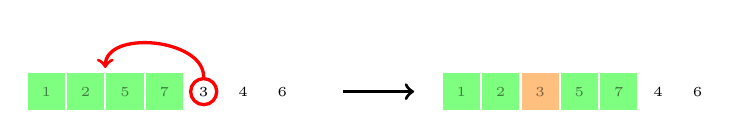
\begin{tikzpicture}
    \node[fill=green,opacity=.5,inner sep=5pt] at (0.25,0.25) {\tiny 1};
    \node[fill=green,opacity=.5,inner sep=5pt] at (0.75,0.25) {\tiny 2};
    \node[fill=green,opacity=.5,inner sep=5pt] at (1.25,0.25) {\tiny 5};
    \node[fill=green,opacity=.5,inner sep=5pt] at (1.75,0.25) {\tiny 7};
    \node at (2.25,0.25) {\tiny 3};
    \node at (2.75,0.25) {\tiny 4};
    \node at (3.25,0.25) {\tiny 6};

    \node[draw,very thick,red,circle] at (2.25,0.25) (a) {};
    \draw[->,very thick,red] (a) to [out=90,in=90] (1,0.55);
    \tableau{7}{1};

    \begin{scope}[xshift=150pt]
      \draw[->,very thick] (-1.25, 0.25) -- (-0.35, 0.25);
      \node[fill=green,opacity=.5,inner sep=5pt] at (0.25,0.25) {\tiny 1};
      \node[fill=green,opacity=.5,inner sep=5pt] at (0.75,0.25) {\tiny 2};
      \node[fill=orange,opacity=.5,inner sep=5pt] at (1.25,0.25) {\tiny 3};
      \node[fill=green,opacity=.5,inner sep=5pt] at (1.75,0.25) {\tiny 5};
      \node[fill=green,opacity=.5,inner sep=5pt] at (2.25,0.25) {\tiny 7};
      \node at (2.75,0.25) {\tiny 4};
      \node at (3.25,0.25) {\tiny 6};
      \tableau{7}{1};
    \end{scope}
  \end{tikzpicture}
\end{center}
\begin{itemize}
    \item On peut procéder en trois étapes:
    \begin{enumerate}
        \item sauvegarder l'élément \code{e} à déplacer
        \item décaler les éléments d'une position de manière à créer une place libre à la destination
        \item affecter la valeur de \code{e} à la destination
    \end{enumerate}
% \item Bien entendu, il faut sauvegarder soit l'élément à déplacer, soit celui qui sera écrasé par ce déplacement;
\end{itemize}
\end{frame}

% ----------------------------------------------------------------------------

\begin{frame}[fragile]
 \frametitle{Insertion d'un élément}

% NOTE: ne leur montrer que ce qui est utile pour le tri, et leur faire faire l'autre sens en TD
% NOTE: on peut faire plus simple en procédant par échanges successifs, mais on effectue à ce moment-là plus d'affectations
\begin{pyframe}{}
def insertion(lst, i):
    # sauvegarder l'élément à déplacer
    e = lst[i]
    # décaler les éléments plus grands
    k = i
    while k > 0 and lst[k-1] > e:
        lst[k] = lst[k-1]
        k = k - 1
    # insérer e en position k
    lst[k] = e
\end{pyframe}

% VERSION COMPLETE:
% \begin{block}{Algorithme de réinsertion}
% \begin{PythonSourceCode}
% def insertion(lst, i, j):
%     e = lst[i]
%     if i < j:              # décalage vers la gauche
%         for k in range(i, j):
%             lst[k] = lst[k + 1]
%     else:                  # décalage vers la droite
%         k = i
%         while k > j:
%             lst[k] = lst[k - 1]
%             k = k - 1
%     lst[j] = e
% \end{PythonSourceCode}
% \end{block}
% \end{frame}

% ----------------------------------------------------------------------------

% \begin{frame}[fragile]
%  \frametitle{Le tri par insertion}
% \begin{itemize}
%     \item On peut donc écrire la fonction suivante en Python:
% \end{itemize}
% TODO environnement algorithme
\begin{pyframe}{}
def tri_insertion(lst):
    for i in range(1, len(lst)):
        insertion(lst, i)
\end{pyframe}
\end{frame}


\begin{frame}
  \frametitle{Complexité du tri par insertion}

  \begin{itemize}
  \item Pour chaque valeur de \code{i} entre \code{1} et \code{n-1} :
    \begin{itemize}
    \item Entre 1 et \code{i-1} comparaisons
    \item Entre 0 et \code{i} affectations
    \end{itemize}
  \item Nombre de comparaisons au pire (liste décroissante) :
    \[
    \sum_{i=0}^{n-2} n-i-1 = \sum_{i=1}^{n-1} i = \frac{n(n-1)}{2} \in \defterm{O(n^2)}
    \]
  \item Nombre d'affectations au pire : $O(n^2)$ (calcul similaire)

  \item Meilleur cas : $O(n)$ sur liste croissante (aucun décalage)

  \item Amélioration possible : chercher la position finale de chaque
    élément par dichotomie sur le début de la liste\\
    (ne change pas le nombre d'affectations nécessaire)
  \end{itemize}
\end{frame}


\subsection{Tri par pivot / tri rapide}

\begin{frame}
    \frametitle{Autres algorithmes de tris}
\begin{itemize}
    \item Les algorithmes de tri déjà présentés ont une complexité prohibitive
    \item On va voir maintenant des algorithmes plus performants
    \begin{enumerate}
        \item le \defterm{tri rapide}
        \item le \defterm{tri fusion}
    \end{enumerate}
\end{itemize}
\end{frame}

% -----------------------------------------------------------------------------
\begin{frame}
    \frametitle{Echauffement: le tri pair / impair}
\begin{itemize}
    \item A titre d'échauffement, essayons de résoudre le problème suivant:
\end{itemize}
  \begin{probleme}[tri pair / impair]\small
    \textbf{Données:} une liste \code{lst} de naturels\\
    \textbf{Objectif:} mettre les éléments pairs de \code{lst} au début et les impairs à la fin
  \end{probleme}
\begin{itemize}
    \item Comment résoudre ce problème de manière efficace?
\end{itemize}
\end{frame}

% TODO: il y a sûrement plusieurs options possibles, si d'autres options intermédiaires vous semblent intéressantes
% d'un point de vue pédagogique, n'hésitez pas

% -----------------------------------------------------------------------------
\begin{frame}
    \frametitle{Echauffement: le tri pair / impair}
\begin{itemize}
    \item Une solution possible: parcourir la liste simultanément avec deux curseurs \code{c1} et \code{c2}
    \item Les deux curseurs progressent l'un vers l'autre au départ des extrémités
    \item A chaque fois qu'on tombe sur un couple (\code{lst[c1]}, \code{lst[c2]}) d'éléments mal placés, on les échange
\end{itemize}
\vfill
    \begin{center}
\begin{tikzpicture}
\tableau{16}{1};
\node (c1) at (0, -.5) {c1};
\node (c2) at (8, -.5) {c2};

\draw[>=stealth,->] (0,-0.25) to (3, -.25);
\draw[>=stealth,->] (8,-0.25) to (5, -.25);
\end{tikzpicture}
    \end{center}
\end{frame}

% Exemple à dérouler sur : [7, 7, 10, 0, 1, 0, 9, 9, 5, 10, 8, 5, 3, 10, 5, 0]
\begin{frame}
 \frametitle{Le tri pair / impair en action}

% \begin{itemize}
%     \item Avant de présenter l'algorithme, illustrons son action sur un exemple simple:
\begin{exemple}
\bigskip
\centering
\begin{tikzpicture}
\node (c1) at (0, -1) {curseur 1};
\node (c2) at (8, -1) {curseur 2};

% Etapes pour les curseurs:
\only<1-2> {
    \draw[>=stealth,->] (c1) to (.25, -.05);
    \draw[>=stealth,->] (c2) to (7.75, -.05);
}

\only<3-4> {
    \draw[>=stealth,->] (c1) to (.75, -.05);
    \draw[>=stealth,->] (c2) to (6.75, -.05);
}

\only<5-6> {
    \draw[>=stealth,->] (c1) to (2.25, -.05);
    \draw[>=stealth,->] (c2) to (5.25, -.05);
}

\only<7-8> {
    \draw[>=stealth,->] (c1) to (3.25, -.05);
    \draw[>=stealth,->] (c2) to (4.75, -.05);
}

\only<9> {
    \draw[>=stealth,->] (c1) to (3.75, -.05);
    \draw[>=stealth,->] (c2) to (3.25, -.05);
}

% Affichage en vert des préfixes et suffixes auxquels on ne touchera plus:
\only<1>{
    \node[fill=red,opacity=.5,inner sep=7pt] at (0.25, 0.25) {};
    \node[fill=red,opacity=.5,inner sep=7pt] at (7.75, 0.25) {};
}

\uncover<2->{
    % préfixe
    \node[fill=green,opacity=.5,inner sep=7pt] at (0.25, 0.25) {};
    % suffixe
    \node[fill=green,opacity=.5,inner sep=7pt] at (7.75, 0.25) {};
}

\uncover<3->{
    % préfixe
    % suffixe
    \node[fill=green,opacity=.5,inner sep=7pt] at (7.25, 0.25) {};
}

\only<3>{
    \node[fill=red,opacity=.5,inner sep=7pt] at (0.75, 0.25) {};
    \node[fill=red,opacity=.5,inner sep=7pt] at (6.75, 0.25) {};
}

\uncover<4->{
    % préfixe
    \foreach \abscisse in {0.75}
        \node[fill=green,opacity=.5,inner sep=7pt] at (\abscisse, 0.25) {};
    % suffixe
    \foreach \abscisse in {6.75}
        \node[fill=green,opacity=.5,inner sep=7pt] at (\abscisse, 0.25) {};
}

\uncover<5->{
    % préfixe
    \foreach \abscisse in {1.25, 1.75}
        \node[fill=green,opacity=.5,inner sep=7pt] at (\abscisse, 0.25) {};
    % suffixe
    \foreach \abscisse in {6.25, 5.75}
        \node[fill=green,opacity=.5,inner sep=7pt] at (\abscisse, 0.25) {};
}

\only<5>{
    \node[fill=red,opacity=.5,inner sep=7pt] at (2.25, 0.25) {};
    \node[fill=red,opacity=.5,inner sep=7pt] at (5.25, 0.25) {};
}

\uncover<6->{
    % préfixe
    \foreach \abscisse in {2.25}
        \node[fill=green,opacity=.5,inner sep=7pt] at (\abscisse, 0.25) {};
    % suffixe
    \foreach \abscisse in {5.25}
        \node[fill=green,opacity=.5,inner sep=7pt] at (\abscisse, 0.25) {};
}

\only<7>{
    \node[fill=red,opacity=.5,inner sep=7pt] at (3.25, 0.25) {};
    \node[fill=red,opacity=.5,inner sep=7pt] at (4.75, 0.25) {};
}

\uncover<7->{
    % préfixe
    \foreach \abscisse in {2.75}
        \node[fill=green,opacity=.5,inner sep=7pt] at (\abscisse, 0.25) {};
    % suffixe
}

\uncover<8->{
    % préfixe
    \foreach \abscisse in {3.25}
        \node[fill=green,opacity=.5,inner sep=7pt] at (\abscisse, 0.25) {};
    % suffixe
    \foreach \abscisse in {4.75}
        \node[fill=green,opacity=.5,inner sep=7pt] at (\abscisse, 0.25) {};
}

\uncover<9>{
    \foreach \abscisse in {3.75, 4.25}
        \node[fill=green,opacity=.5,inner sep=7pt] at (\abscisse, 0.25) {};
}


% Etapes pour le contenu :
\tableau{16}{1};

\only<1>{
\foreach[count=\i] \valeur in {7, 7, 10, 0, 1, 0, 9, 9, 5, 10, 8, 5, 3, 10, 5, 0}
    \node at (-0.25+\i/2,0.25) {\tiny \valeur};
}

\only<2-3>{
\foreach[count=\i] \valeur in {0, 7, 10, 0, 1, 0, 9, 9, 5, 10, 8, 5, 3, 10, 5, 7}
    \node at (-0.25+\i/2,0.25) {\tiny \valeur};
}

\only<4-5>{
\foreach[count=\i] \valeur in {0, 10, 10, 0, 1, 0, 9, 9, 5, 10, 8, 5, 3, 7, 5, 7}
    \node at (-0.25+\i/2,0.25) {\tiny \valeur};
}

\only<6-7>{
\foreach[count=\i] \valeur in {0, 10, 10, 0, 8, 0, 9, 9, 5, 10, 1, 5, 3, 7, 5, 7}
    \node at (-0.25+\i/2,0.25) {\tiny \valeur};
}

\only<8->{
\foreach[count=\i] \valeur in {0, 10, 10, 0, 8, 0, 10, 9, 5, 9, 1, 5, 3, 7, 5, 7}
    \node at (-0.25+\i/2,0.25) {\tiny \valeur};
}

\end{tikzpicture}

\end{exemple}

\begin{itemize}
\item<9> L'algorithme s'arrête quand les curseurs se croisent
\end{itemize}

\end{frame}

% -----------------------------------------------------------------------------

\begin{frame}[fragile]
    \frametitle{Le tri pair / impair en Python}

{
\scriptsize
\begin{pyframe}{}
def pair_impair(lst):
    curseur1, curseur2 = 0, len(lst) - 1
    while curseur1 <= curseur2:
        # repérer le premier élément impair en partant du début
        while curseur1 <= curseur2 and lst[curseur1] % 2 == 0:
            curseur1 += 1

        # repérer le premier élément pair en partant de la fin
        while curseur1 <= curseur2 and lst[curseur2] % 2 != 0:
            curseur2 -= 1

        # si nécessaire, procéder à l'échange
        if curseur1 < curseur2:
            lst[curseur1], lst[curseur2] = lst[curseur2], lst[curseur1]
            curseur1 += 1
            curseur2 -= 1
\end{pyframe}
}
\begin{itemize}
\item Complexité?  \pause \defterm{Temps $O(n)$, espace
    $O(1)$}
\end{itemize}

\end{frame}

% -----------------------------------------------------------------------------

\begin{frame}
    \frametitle{Généralisation}
\begin{itemize}
    \item On peut utiliser ce principe pour \defterm{trier} la liste
    \item Au lieu de se contenter de mettre les pairs au début et les
      impairs à la fin, on peut mettre les éléments inférieurs à une
      certaine valeur avant elle et les autres après elle
    \item Ce principe est à la base du \defterm{tri rapide}
\end{itemize}
\end{frame}

% -----------------------------------------------------------------------------

\begin{frame}
    \frametitle{Le tri rapide}
\begin{itemize}
    \item Principe du tri rapide:
    \begin{enumerate}
    \item Sélectionner un \defterm{pivot}, c'est-à-dire une
      \defterm{valeur} \texttt{p} de référence dans la liste (par
      exemple la première)
    \item \defterm{Partitionner} la liste :
      \begin{itemize}
      \item Toutes les valeurs inférieures à \texttt{p} se retrouvent
        avant \texttt{p}
      \item Toutes les valeurs supérieures à \texttt{p} se retrouvent
        après \texttt{p}
      \end{itemize}
    \item Recommencer récursivement sur les deux parties de liste
      (avant et après le pivot)
    \end{enumerate}
\end{itemize}

\end{frame}

% -----------------------------------------------------------------------------
\begin{frame}
    \frametitle{Le tri rapide}
\begin{exemple}
\centering
\begin{tikzpicture}
\visible<1-5> {
  \node (c1) at (0, -1) {curseur 1};
  \node (c2) at (4, -1) {curseur 2};
}

% Etapes pour les curseurs:
\only<1> {
    \draw[>=stealth,->] (c1) to (.75, -.05);
    \draw[>=stealth,->] (c2) to (3.75, -.05);
}

\only<2-3> {
    \draw[>=stealth,->] (c1) to (1.75, -.05);
    \draw[>=stealth,->] (c2) to (3.25, -.05);
}

\only<4-5> {
    \draw[>=stealth,->] (c1) to (2.25, -.05);
    \draw[>=stealth,->] (c2) to (1.75, -.05);
}

\only<1-4>{
    %pivot
    \node[fill=blue,opacity=.5,inner sep=7pt] at (0.25, 0.25) {};
}

% Affichage en vert des préfixes et suffixes auxquels on ne touchera plus:
\only<2-4>{
    % préfixe
    \foreach \abscisse in {0.75, 1.25}
        \node[fill=green,opacity=.5,inner sep=7pt] at (\abscisse, 0.25) {};
    % suffixe
    \foreach \abscisse in {3.75}
        \node[fill=green,opacity=.5,inner sep=7pt] at (\abscisse, 0.25) {};
}

\only<3>{
    % échange
    \foreach \abscisse in {1.75, 3.25}
        \node[fill=red,opacity=.5,inner sep=7pt] at (\abscisse, 0.25) {};
}


\only<4>{
    \foreach \abscisse in {1.75, 2.25, 2.75, 3.25}
        \node[fill=green,opacity=.5,inner sep=7pt] at (\abscisse, 0.25) {};
}

% Placement du pivot

\only<5> {
  \node[fill=red,opacity=.5,inner sep=7pt] at (0.25, 0.25) {};
  \node[fill=blue,opacity=.5,inner sep=7pt] at (1.75, 0.25) {};
}
\only<6> {
  \node[fill=blue,opacity=.5,inner sep=7pt] at (1.75, 0.25) {};
}

% Etapes pour le contenu:
\tableau{8}{1};

\only<1-2>{
\foreach[count=\i] \valeur in {3, 2, 1, 6, 4, 7, 2, 5}
    \node at (-0.25+\i/2,0.25) {\tiny \valeur};
}

\only<3-4>{
\foreach[count=\i] \valeur in {3, 2, 1, 2, 4, 7, 6, 5}
    \node at (-0.25+\i/2,0.25) {\tiny \valeur};
}

\only<5->{
\foreach[count=\i] \valeur in {2, 2, 1, 3, 4, 7, 6, 5}
    \node at (-0.25+\i/2,0.25) {\tiny \valeur};
}

\end{tikzpicture}
\end{exemple}

\begin{enumerate}
    \item On partitionne avec le premier élément comme pivot
    \item<5-> On place le pivot à la ``frontière''
    \item<6-> On trie les deux zones récursivement par le même principe
\end{enumerate}

\end{frame}

% -----------------------------------------------------------------------------

\begin{frame}[fragile]
    \frametitle{Calcul de la partition}
\begin{itemize}
    \item L'algorithme est très similaire au tri pair / impair;
    \begin{itemize}
        \item avant: pairs à gauche, impairs à droite;
        \item maintenant: $x\leq$ \code{p} à gauche, $y>$ \code{p} à droite;
    \end{itemize}
\end{itemize}
\scriptsize
\begin{pyframe}{}
def partition(lst, debut, fin):
    curseur1, curseur2 = debut + 1, fin

    while curseur1 <= curseur2:
        while curseur1 <= curseur2 and lst[curseur1] <= lst[debut]:
            curseur1 += 1

        while lst[curseur2] > lst[debut]:
            curseur2 -= 1

        if curseur1 < curseur2:  # si nécessaire, procéder à l'échange
            lst[curseur1], lst[curseur2] = lst[curseur2], lst[curseur1]
            curseur1 += 1
            curseur2 -= 1

    lst[debut], lst[curseur2] = lst[curseur2], lst[debut]
    return curseur2  # la position finale du pivot servira plus tard
\end{pyframe}

\end{frame}


\begin{frame}[fragile]
\frametitle{Le tri rapide en Python}

\footnotesize
\begin{pyframe}{}
def tri_rapide(lst, debut=0, fin=None):
    if fin is None:
        fin = len(lst) - 1

    if debut < fin:
        # partition entre debut et fin
        pivot = partition(lst, debut, fin)

        # tri de la zone entre debut et pivot
        tri_rapide(lst, debut, pivot - 1)

        # tri de la zone entre pivot et fin
        tri_rapide(lst, pivot + 1, fin)
\end{pyframe}
\end{frame}


\begin{frame}
  \frametitle{Complexité du tri rapide}

  \begin{itemize}
  \item Complexité du partitionnement : \defterm{$O(n)$}

    \medskip

  \item Pire cas : élément minimal ou maximal comme pivot
    \begin{itemize}
    \item Une partie à 0 éléments, l'autre à $n-1$ éléments
    \item Mêmes calculs que pour les tris naïfs : \defterm{$O(n^2)$}
    \end{itemize}

    \medskip

  \item Cas le plus favorable : partition en deux moitiés égales
    \begin{itemize}
    \item Nombre d'appels récursifs en $O(\log n)$
    \item Au $k^e$ niveau de récursion on partitionne environ $2^k$
      listes de taille environ $n / 2^k$, coût total $O(n)$
    \item Coût total : \defterm{$O(n \log n)$}
    \end{itemize}

    \medskip

  \item En moyenne : on peut montrer qu'on obtient
    \defterm{$O(n \log n)$}
  \end{itemize}
\end{frame}


\begin{frame}
  \frametitle{Tri par pivot}

  \begin{itemize}
  \item Pire cas du tri par pivot : liste déjà triée

    \medskip

  \item Problème : en pratique cas très fréquent !

    \medskip

  \item (au moins) 2 solutions :
    \begin{itemize}
    \item Mélanger la liste avant de commencer (\code{random.shuffle},
      détails à suivre)
    \item Choisir un pivot au hasard avant de partitionner
    \end{itemize}
  \end{itemize}

\end{frame}


\begin{frame}[fragile]
\frametitle{Le tri rapide en Python}

\scriptsize
\begin{pyframe}{}
def tri_rapide(lst, debut=0, fin=None):
    if fin is None:
        fin = len(lst) - 1

    if debut < fin:
        # choix d'un pivot aléatoire et placement en debut
        pivot = random.randint(debut, fin)
        lst[debut], lst[pivot] = lst[pivot], lst[debut]

        # partition entre debut et fin
        pivot = partition(lst, debut, fin)

        # tri de la zone entre debut et pivot
        tri_rapide(lst, debut, pivot - 1)

        # tri de la zone entre pivot et fin
        tri_rapide(lst, pivot + 1, fin)
\end{pyframe}
\end{frame}


\subsection{Tri par fusion}

\begin{frame}
    \frametitle{Le tri fusion}
\begin{itemize}
    \item
Ce tri se d\'ecrit facilement r\'ecursivement:\\
\begin{itemize}
\item Si la liste contient 0 ou 1 élément, elle est triée
\item Sinon :
\begin{enumerate}
    \item On la divise en deux listes de tailles égales
    \item On trie les deux sous-listes
    \item On fusionne le résultat à l'aide d'une liste auxiliaire
    \item On recopie la liste auxiliaire dans la liste d'origine
\end{enumerate}
\end{itemize}
\end{itemize}
\begin{center}
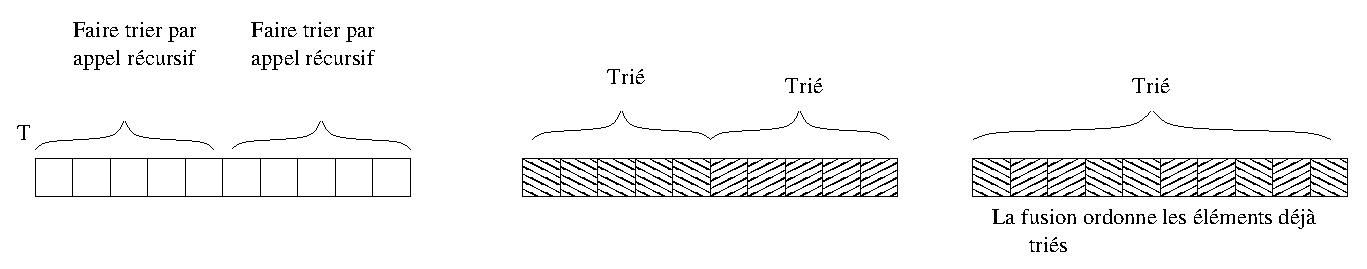
\includegraphics[scale=.5]{fusion.eps}
\end{center}
\end{frame}

\begin{frame}
\frametitle{La partie fusion}

\begin{itemize}
    \item Algorithme de fusion de listes triées :
\begin{itemize}
    \item On utilise deux curseurs parcourant
      \code{lst1} et \code{lst2} en parallèle dans le même sens
    \item À chaque étape, on ajoute \code{min(lst1[c1], lst2[c2])} au
      résultat
    \item Si une des listes est épuisée on recopie la fin de l'autre
\end{itemize}

\medskip

\item Ici, on va travailler sur deux \defterm{portions voisines} d'une
  même liste \code{lst}
  \begin{itemize}
  \item Il est suffisant de travailler avec des indices
  \item Une fois le résultat obtenu, on le recopie sur la portion
    correspondante de \code{lst}
  \end{itemize}
\end{itemize}



\end{frame}


\begin{frame}[fragile]
\frametitle{La partie ``fusion''}

\scriptsize
\begin{pyframe}{}
def fusionner(lst, debut, milieu, fin):
    aux = []
    curseur1, curseur2 = debut, milieu + 1
    for k in range(debut, fin + 1):
        # si une des deux sous-listes a été copiée, copier l'autre
        if curseur1 > milieu:
            aux.append(lst[curseur2])
            curseur2 += 1
        elif curseur2 > fin:
            aux.append(lst[curseur1])
            curseur1 += 1
        # sinon, copier min(lst[curseur1], lst[curseur2])
        elif lst[curseur1] < lst[curseur2]:
            aux.append(lst[curseur1])
            curseur1 += 1
        else:
            aux.append(lst[curseur2])
            curseur2 += 1
    # on recopie la liste auxiliaire sur la liste à trier
    lst[debut:fin+1] = aux
\end{pyframe}
\end{frame}

\begin{frame}[fragile]
\frametitle{La partie ``tri''}

% \begin{itemize}
%     \item Une fois la partie fusion écrite, le tri se résume à ceci:
% \end{itemize}
\footnotesize
\begin{pyframe}{}
def tri_fusion(lst, debut, fin):
    # plus que 0 ou 1 élément à trier
    if debut >= fin:
        return

    # partitionner en deux-sous listes
    milieu = debut + (fin - debut) // 2

    # les trier
    tri_fusion(lst, debut, milieu)
    tri_fusion(lst, milieu+1, fin)

    # les fusionner
    fusionner(lst, debut, milieu, fin)
\end{pyframe}

\end{frame}

\begin{frame}
    \frametitle{Complexité}

  \begin{itemize}
  \item Complexité de la fusion: \defterm{$O(n)$}

    \medskip

  \item Même idée que pour le cas favorable du tri par pivot

    \medskip

  \item Dans tous les cas : partition en deux moitiés égales
    \begin{itemize}
    \item Profondeur max d'appels récursifs imbriqués : $O(\log n)$
    \item Au $k^e$ niveau de récursion on fusionne $2^k$
      listes de taille environ $n / 2^k$, coût total $O(n)$
    \item Coût total : \defterm{$O(n \log n)$}
    \end{itemize}

  \item Algorithme (asymptotiquement) \defterm{optimal} mais plus de mémoire
  utilisée que tri par pivot

  \item Tri \defterm{stable} (des éléments égaux restent dans le même ordre)
  \end{itemize}
\end{frame}


\subsection{Le tri de Python}
\label{sub:le_tri_de_python}

\begin{frame}
\frametitle{Le tri de Python}

Méthode \code{sort} : tri sur place de \code{list}
\begin{itemize}
  \item Algo hybride entre tri par fusion et tri par insertion (\emph{Timsort})
  \item Stable, $O(n \log n)$ en temps (au pire et en moyenne), $O(n)$ en espace
  \item Utilisé par d'autres langages de programmation (par ex. Java)
  \item \textbf{Attention :} trie sur place, ne renvoie pas de liste !
  \item Possibilité de trier selon un critère donné (\code{key=f}), ou à l'envers (\code{reverse=True})
\end{itemize}

\medskip

Tri sans modification de la liste : fonction \code{sorted}
\end{frame}

\begin{frame}[fragile]
\frametitle{Le tri de Python}

\scriptsize
\begin{python}
>>> lst = ["Chennai", "Mumbai", "Kochi", "Delhi", "Calcutta", "Amritsar"]
>>> lst.sort()
>>> print(lst)
['Amritsar', 'Calcutta', 'Chennai', 'Delhi', 'Kochi', 'Mumbai']

>>> lst.sort(reverse=True)
>>> print(lst)
['Mumbai', 'Kochi', 'Delhi', 'Chennai', 'Calcutta', 'Amritsar']

>>> lst.sort(key=len)
>>> print(lst)
['Kochi', 'Delhi', 'Mumbai', 'Chennai', 'Calcutta', 'Amritsar']

>>> def derniere_lettre(s):
...    return s[-1]
...
>>> sorted(lst, key=derniere_lettre)
['Calcutta', 'Kochi', 'Delhi', 'Mumbai', 'Chennai', 'Amritsar']
\end{python}

\end{frame}


\section{Variations autour du tri}


\subsection{Mélange de liste} % (fold)
\label{sub:mélange_de_liste}

\begin{frame}[fragile]
\frametitle{Mélange de liste}

On a vu comment trier une liste, mais comment la mélanger uniformément ?

\begin{pyframe}{Première tentative :}
from random import randrange

def melange(lst):
    for i in range(len(lst)):
        k = randrange(len(lst))
        lst[i], lst[k] = lst[k], lst[i]
\end{pyframe}

\defterm{Exercice :} Quelle est la fréquence d'apparition de chaque résultat possible sur une liste de longueur 3 ?

\end{frame}

\begin{frame}[fragile]
\frametitle{Mélange de liste}

\begin{pyframe}{}
from random import randrange
def melange(lst):
    for i in range(len(lst)):
        k = randrange(len(lst))
        lst[i], lst[k] = lst[k], lst[i]
\end{pyframe}

\defterm{Buggé !!!}
\begin{itemize}
  \item Combien de permutations possibles ? $n!$
  \item Combien d'exécutions possibles de l'algorithme ? $n^n$ (beaucoup plus)
  \item $n^n$ n'est pas divisible par $n!$ en général $\rightarrow$ répartition égale impossible
\end{itemize}

\end{frame}

\begin{frame}[fragile]
\frametitle{Mélange de liste}

\begin{pyframe}{Seconde tentative}
def melange(lst):
    for i in range(len(lst)-1):
        k = randrange(i, len(lst))  # changement ici !
        lst[i], lst[k] = lst[k], lst[i]
\end{pyframe}

On peut raisonner à l'envers pour comprendre :
\begin{itemize}
  \item À chaque étape on "devine" l'élément qui était en position \code{i} avant de trier
  \item Les éléments de rang $< \code{i}$ sont déjà fixés, donc on le nes considère pas
  \item Une fois chaque élément fixé, on a fini
  \item Complexité : \pause $O(n)$
\end{itemize}

\end{frame}



% subsection mélange_de_liste (end)

\subsection{Recherche de la médiane} % (fold)
\label{sub:recherche_de_la_médiane}


\begin{frame}
\frametitle{Recherche de la médiane}

\begin{beamerboxesrounded}{Problème de recherche de la médiane}
Donnée : une liste de $n$ éléments comparables\\
Résultat : l'élément médian de la liste
\end{beamerboxesrounded}

\color{gray}{\small (Médiane : autant d'éléments supérieurs que d'éléments inférieurs)}

\begin{itemize}
  \item Algorithme naïf : calculer $\lfloor n/2 \rfloor$ fois le plus petit élément parmi les éléments restants
  \item Complexité : \pause $O(n^2)$. Peut-on faire mieux ? \pause
  \item Idée : si on partitionne selon un pivot, l'élément médian est dans la partie qui contient plus de $n/2$ éléments...
\end{itemize}

\defterm{Exercice :} écrire une fonction efficace de recherche de la médiane

\end{frame}

\begin{frame}[fragile]
\frametitle{Recherche de la médiane}

\begin{beamerboxesrounded}{Problème de recherche du $k$è plus petit}
Donnée : une liste de $n$ éléments comparables\\
Résultat : le $k$è plus petit élément de la liste
\end{beamerboxesrounded}

{\footnotesize
\begin{python}
def plus_petit(lst, k):
    debut = 0
    fin = len(lst)-1
    while True:
        p = randint(debut, fin)
        p = partitionne(lst, debut, p, fin)
        if p == k:
            return lst[k]
        elif p < k:
            debut = p+1
        else:
            fin = p-1
\end{python}
}

Complexité : \pause $O(n)$ en temps et $O(1)$ en espace (en moyenne !)

\end{frame}

% subsection recherche_de_la_médiane (end)

\end{document}
